\documentclass{memoir}

\usepackage{calc}
\usepackage{hyperref}

%%% Page geometry
\usepackage[
  paperwidth=8.5in,
  paperheight=8.5in,
  layoutwidth=8.5in,
  layoutheight=8.5in,
  vmargin=0.5in,
  outer=0.5in,
  inner=0.75in,
  includeheadfoot,
  twoside
]{geometry}

%%% Font
\usepackage{fontspec}
\setmainfont{Gentium Book Basic}
\newfontfamily\titlefamily{Ubuntu}
\newfontface\titlefont{Ubuntu}
\newfontface\urlfont{Ubuntu Mono}

%%% Graphics
\usepackage{graphicx}

%%% Table of contents
\renewcommand{\contentsname}{\titlefamily FOOD}
% flushright chapter numbers
\renewcommand{\cftchapterfont}{\normalfont\titlefamily\bfseries}
\renewcommand{\cftsectionfont}{\normalfont\titlefamily}
\setlength{\cftbeforechapterskip}{1.6ex}
\setlength{\cftbeforesectionskip}{0.75ex}
\renewcommand{\cftdot}{\small{$\cdot$}}
\renewcommand{\cftchapterdotsep}{10000}
\renewcommand{\cftsectiondotsep}{3}
\renewcommand*\tocheadstart{}{}

%%% Headers and chapters
\let\footruleskip\undefined
\DisemulatePackage{setspace}
\usepackage[pagestyles]{titlesec}
\usepackage{fancyhdr}
\setlength{\headheight}{15.2pt}
% arcana style with fancy headers and chapter headings
\fancypagestyle{fancyplain}{
  % headers
  \fancyhf{}
  \fancyhf[FRO,FLE]{\titlefamily\thepage}
  \fancyhf[HLE]{\titlefamily\chaptertitle}
  \fancyhf[HRO]{\titlefamily MEALTIME WITH MADDY}

  %%% With inner headers
  % \fancyhf[HLE,HRO]{\titlefamily\textit{Arcana}}
  % \fancyhf[HLO]{\pfdfamily\itshape\arcstoryauthor}
  % \fancyhf[HRE]{\titlefamily\ifthenelse{\equal{\arcsubheading}{}}{\chaptertitle}{\chaptertitle\normalfont\ --- {\pfdfamily\arcsubheading}}}
  \renewcommand{\headrulewidth}{0.5pt}
  \renewcommand{\chapterheadstart}{}
  \renewcommand{\printchaptername}{}
  \renewcommand{\chapternamenum}{}
  \renewcommand{\printchapternum}{}
  \renewcommand{\afterchapternum}{}
  \renewcommand{\printchaptertitle}[1]{%
  \titlefamily\raggedright\Huge{##1}}
  \renewcommand{\afterchaptertitle}{%
  \vskip\onelineskip \hrule\vskip\onelineskip}
  \setbeforesecskip{1ex}
  \setaftersecskip{1ex}
  \setlength{\parskip}{0pt}
}
\fancypagestyle{afterword}{
  % headers - same for arcana pagestyle
  \fancyhf{}
  \fancyhf[FRO,FLE]{\titlefamily\thepage}
  \fancyhf[HLE,HRO]{\titlefamily MEALTIME WITH MADDY}
  % chapter headings with card names - same for arcana pagestyle
  \renewcommand{\headrulewidth}{0.5pt}
  \renewcommand{\chapterheadstart}{}
  \renewcommand{\printchaptername}{}
  \renewcommand{\chapternamenum}{}
  \renewcommand{\printchapternum}{}
  \renewcommand{\afterchapternum}{}
  % this is the only changed command from arcana: remove \thechapter from chapter header
  \renewcommand{\printchaptertitle}[1]{%
  \titlefamily\raggedright\Huge{\hspace{2em} ##1}}
  \renewcommand{\afterchaptertitle}{%
  \vskip\onelineskip \hrule\vskip\onelineskip}
  \setbeforesecskip{1ex}
  \setaftersecskip{1ex}
}
% plain style with only page num
\fancypagestyle{plain}{
  \fancyhf{}
  \renewcommand{\headrulewidth}{0pt}
  \renewcommand{\footrulewidth}{0pt}
  \fancyhf[FRO,FLE]{\thepage}
}
% single space after periods
\frenchspacing
% Attempt justification at all costs
\sloppy


\begin{document}
\frontmatter

\pagestyle{empty}
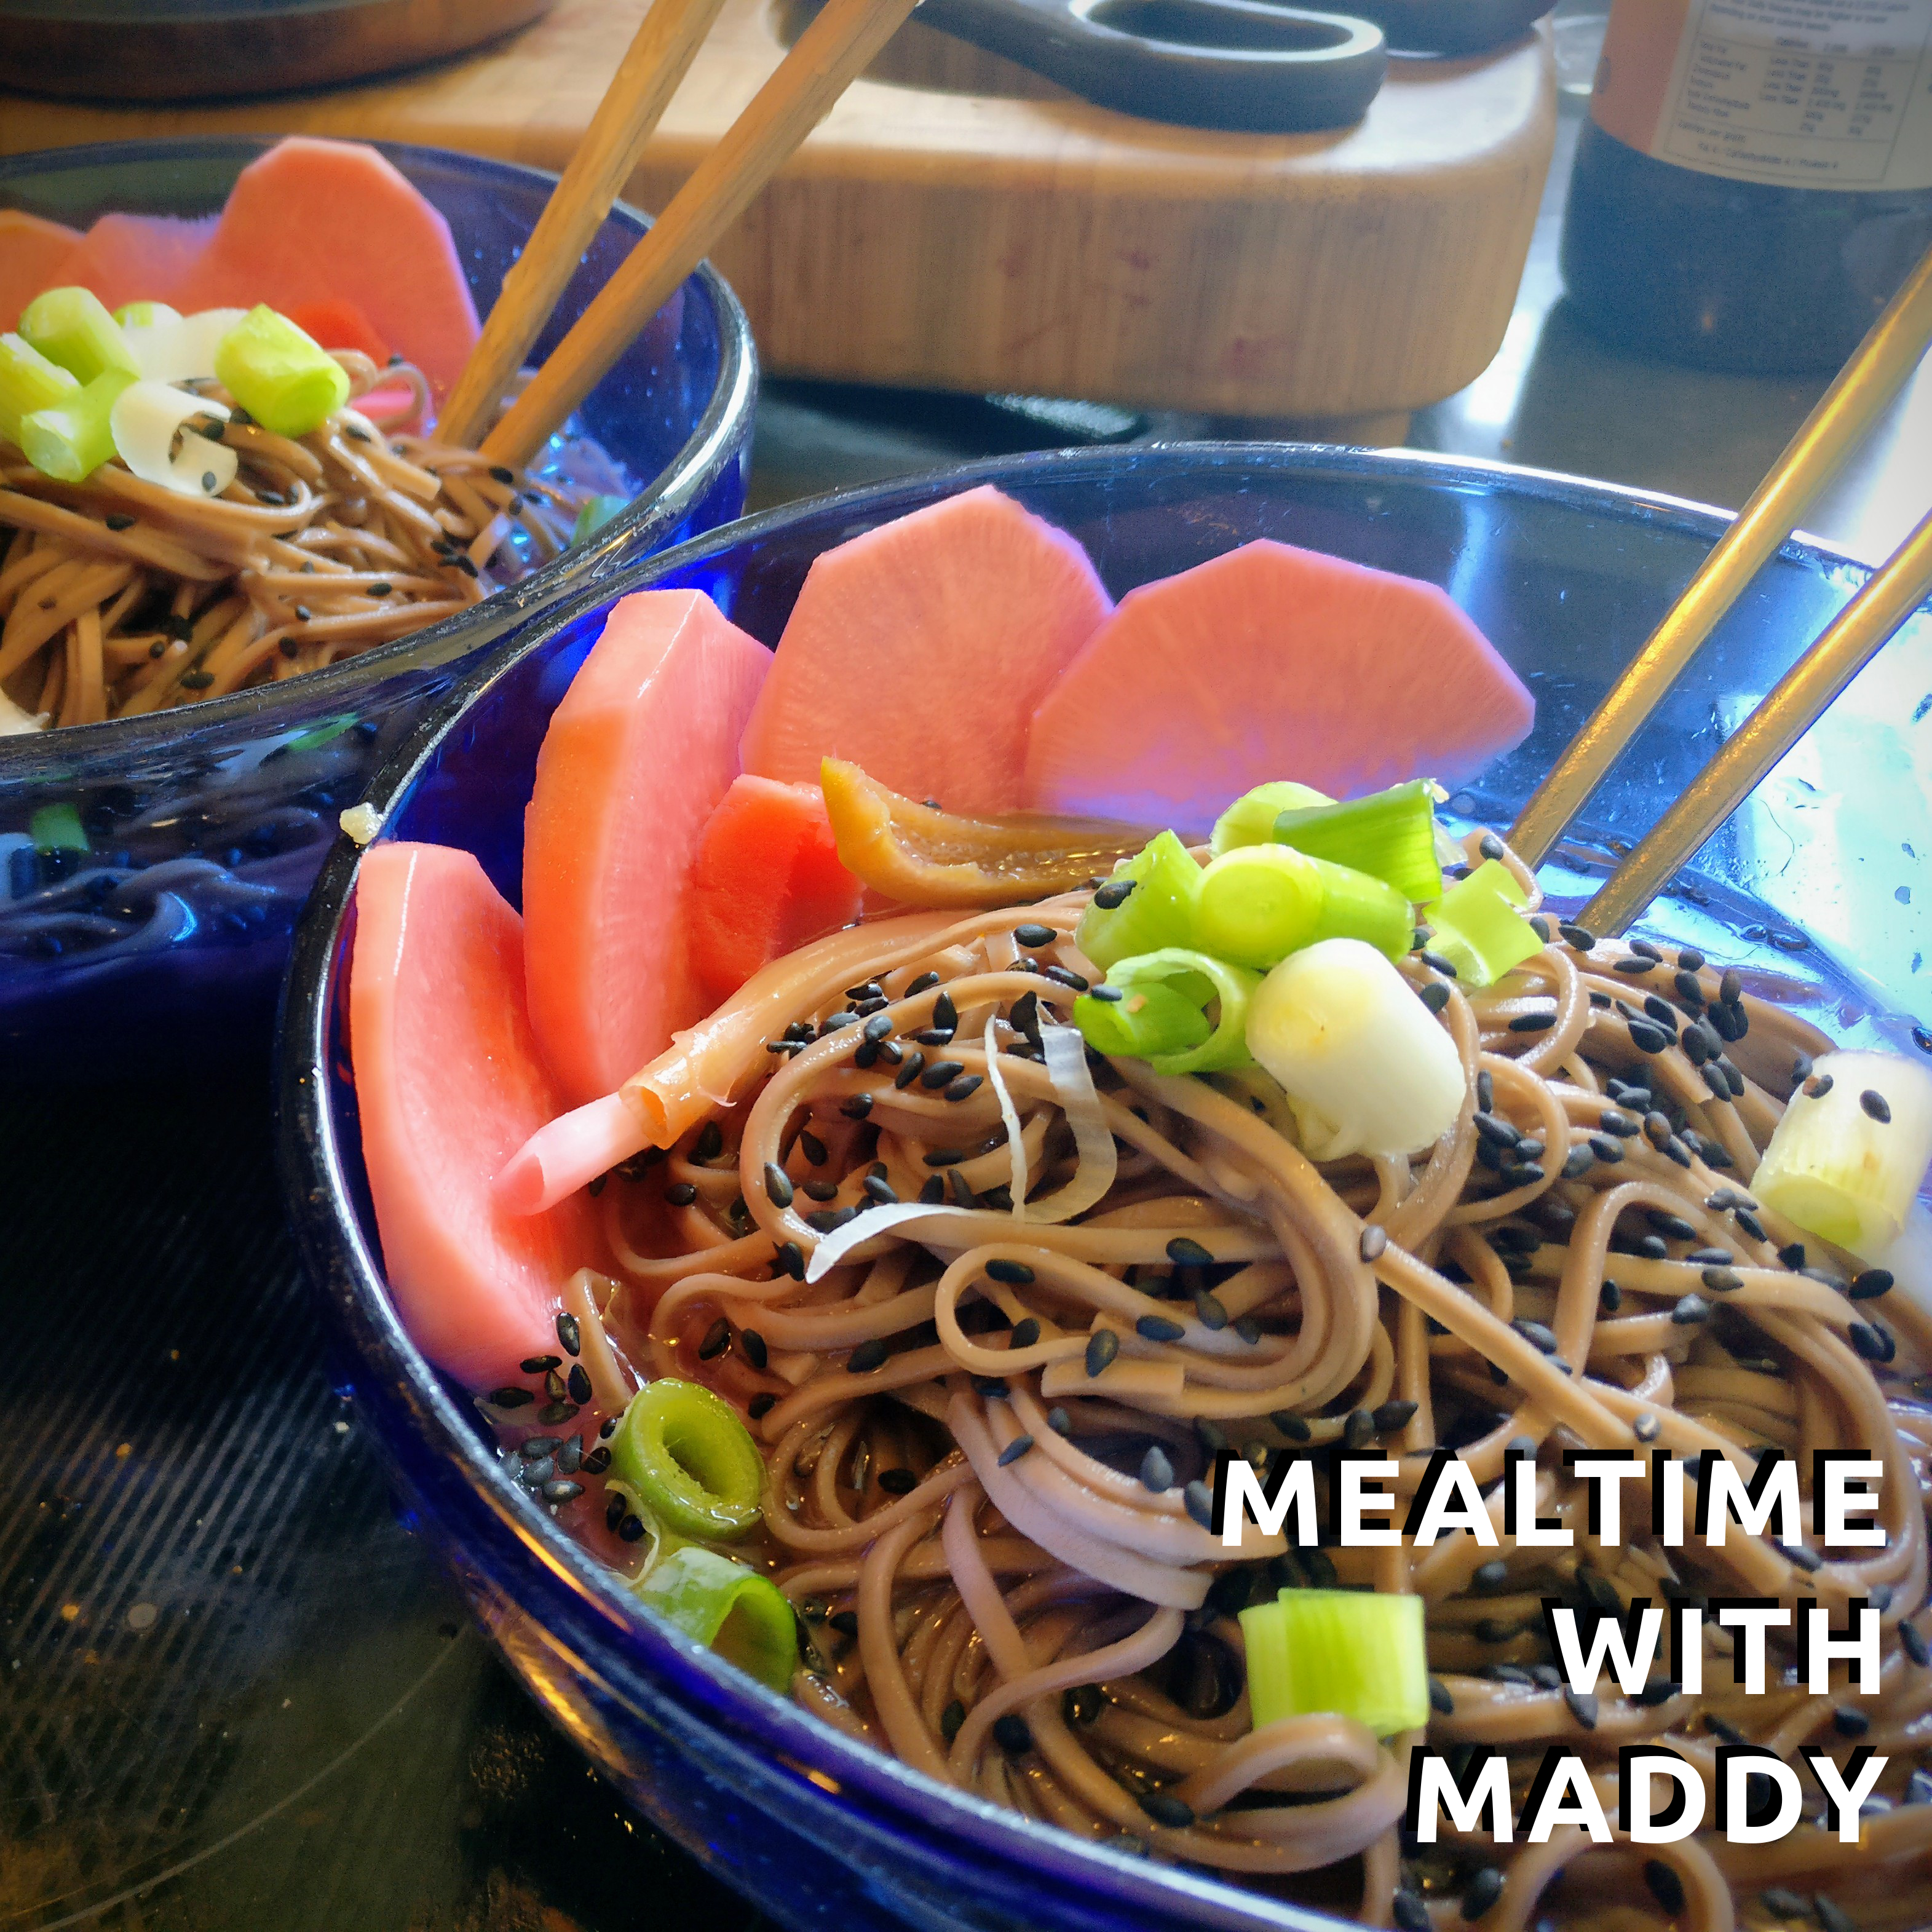
\includegraphics[width=6.5in]{inner-cover.png}
\newpage

\null
\vfill

\titlefont MEALTIME WITH MADDY \copyright\ Madison Scott-Clary, 2017

\vspace{1ex}

This work is licensed under a Creative Commons Attribution-ShareAlike 4.0 International License

\vspace{1ex}

For more information, see \mbox{\urlfont https://creativecommons.org/licenses/by-sa/4.0/}

\vspace{1cm}

This book is part of an evolving project.

To keep up to date and see future recipes and hollering, visit \mbox{\urlfont http://mealtime.with.maddypa.ws}

\vfill
\newpage

\pagestyle{fancyplain}
\tableofcontents*

\normalfont

\chapter*{Dedication}

\begin{verse}
  To the polycule\\
  \vin JD and Robin and Lexy\\
  %To Jenn\\
  To the dogs\\
  \vin Zephyr and Falcon\\
  And to the idea\\
  \vin If not exactly the implementation\\
  \vin \vin Of Twitter.
\end{verse}

\chapter[About]{About}

\mainmatter

\chapter*{Ghee}
\renewcommand{\chaptertitle}{Ghee}
\addcontentsline{toc}{chapter}{\hspace{1.5ex}Ghee}


\chapter*{Bananas Foster}
\renewcommand{\chaptertitle}{Bananas Foster}
\addcontentsline{toc}{chapter}{\hspace{1.5ex}Bananas Foster}

\includegraphics[height=\textwidth-1.3in]{food/bananas-foster/images/hi-res/01.jpg}
\newpage
\includegraphics[width=\textwidth]{food/bananas-foster/images/hi-res/02.jpg}
\newpage
\includegraphics[width=\textwidth]{food/bananas-foster/images/hi-res/03.jpg}
\newpage
\includegraphics[width=\textwidth]{food/bananas-foster/images/hi-res/04.jpg}
\newpage
\includegraphics[width=\textwidth]{food/bananas-foster/images/hi-res/05.jpg}
\newpage
\includegraphics[width=\textwidth]{food/bananas-foster/images/hi-res/06.jpg}
\newpage
\includegraphics[height=\textheight]{food/bananas-foster/images/hi-res/07.jpg}
\newpage
\includegraphics[width=\textwidth]{food/bananas-foster/images/hi-res/08.jpg}
\newpage
\includegraphics[width=\textwidth]{food/bananas-foster/images/hi-res/09.jpg}
\newpage
\includegraphics[width=\textwidth]{food/bananas-foster/images/hi-res/10.jpg}


\chapter*{Preserved Lemons: Part 1}
\renewcommand{\chaptertitle}{Preserved Lemons: Part 1}
\addcontentsline{toc}{chapter}{\hspace{1.5ex}Preserved Lemons: Part 1}


\chapter*{Summer Salad}
\renewcommand{\chaptertitle}{Summer Salad}
\addcontentsline{toc}{chapter}{\hspace{1.5ex}Summer Salad}


\chapter*{Bananas Foster}
\renewcommand{\chaptertitle}{Bananas Foster}
\addcontentsline{toc}{chapter}{\hspace{1.5ex}Bananas Foster}

\includegraphics[height=\textwidth-1.3in]{food/bananas-foster/images/hi-res/01.jpg}
\newpage
\includegraphics[width=\textwidth]{food/bananas-foster/images/hi-res/02.jpg}
\newpage
\includegraphics[width=\textwidth]{food/bananas-foster/images/hi-res/03.jpg}
\newpage
\includegraphics[width=\textwidth]{food/bananas-foster/images/hi-res/04.jpg}
\newpage
\includegraphics[width=\textwidth]{food/bananas-foster/images/hi-res/05.jpg}
\newpage
\includegraphics[width=\textwidth]{food/bananas-foster/images/hi-res/06.jpg}
\newpage
\includegraphics[height=\textheight]{food/bananas-foster/images/hi-res/07.jpg}
\newpage
\includegraphics[width=\textwidth]{food/bananas-foster/images/hi-res/08.jpg}
\newpage
\includegraphics[width=\textwidth]{food/bananas-foster/images/hi-res/09.jpg}
\newpage
\includegraphics[width=\textwidth]{food/bananas-foster/images/hi-res/10.jpg}


\chapter*{Preserved Lemons: Part 2}
\renewcommand{\chaptertitle}{Preserved Lemons: Part 2}
\addcontentsline{toc}{chapter}{\hspace{1.5ex}Preserved Lemons: Part 2}


\chapter*{Bananas Foster}
\renewcommand{\chaptertitle}{Bananas Foster}
\addcontentsline{toc}{chapter}{\hspace{1.5ex}Bananas Foster}

\includegraphics[height=\textwidth-1.3in]{food/bananas-foster/images/hi-res/01.jpg}
\newpage
\includegraphics[width=\textwidth]{food/bananas-foster/images/hi-res/02.jpg}
\newpage
\includegraphics[width=\textwidth]{food/bananas-foster/images/hi-res/03.jpg}
\newpage
\includegraphics[width=\textwidth]{food/bananas-foster/images/hi-res/04.jpg}
\newpage
\includegraphics[width=\textwidth]{food/bananas-foster/images/hi-res/05.jpg}
\newpage
\includegraphics[width=\textwidth]{food/bananas-foster/images/hi-res/06.jpg}
\newpage
\includegraphics[height=\textheight]{food/bananas-foster/images/hi-res/07.jpg}
\newpage
\includegraphics[width=\textwidth]{food/bananas-foster/images/hi-res/08.jpg}
\newpage
\includegraphics[width=\textwidth]{food/bananas-foster/images/hi-res/09.jpg}
\newpage
\includegraphics[width=\textwidth]{food/bananas-foster/images/hi-res/10.jpg}


\chapter*{Bananas Foster}
\renewcommand{\chaptertitle}{Bananas Foster}
\addcontentsline{toc}{chapter}{\hspace{1.5ex}Bananas Foster}

\includegraphics[height=\textwidth-1.3in]{food/bananas-foster/images/hi-res/01.jpg}
\newpage
\includegraphics[width=\textwidth]{food/bananas-foster/images/hi-res/02.jpg}
\newpage
\includegraphics[width=\textwidth]{food/bananas-foster/images/hi-res/03.jpg}
\newpage
\includegraphics[width=\textwidth]{food/bananas-foster/images/hi-res/04.jpg}
\newpage
\includegraphics[width=\textwidth]{food/bananas-foster/images/hi-res/05.jpg}
\newpage
\includegraphics[width=\textwidth]{food/bananas-foster/images/hi-res/06.jpg}
\newpage
\includegraphics[height=\textheight]{food/bananas-foster/images/hi-res/07.jpg}
\newpage
\includegraphics[width=\textwidth]{food/bananas-foster/images/hi-res/08.jpg}
\newpage
\includegraphics[width=\textwidth]{food/bananas-foster/images/hi-res/09.jpg}
\newpage
\includegraphics[width=\textwidth]{food/bananas-foster/images/hi-res/10.jpg}


\chapter*{Preserved Lemons: Part 1}
\renewcommand{\chaptertitle}{Preserved Lemons: Part 1}
\addcontentsline{toc}{chapter}{\hspace{1.5ex}Preserved Lemons: Part 1}


\chapter*{Juk}
\renewcommand{\chaptertitle}{Juk}
\addcontentsline{toc}{chapter}{\hspace{1.5ex}Juk}


\chapter*{Preserved Lemons: Part 2}
\renewcommand{\chaptertitle}{Preserved Lemons: Part 2}
\addcontentsline{toc}{chapter}{\hspace{1.5ex}Preserved Lemons: Part 2}


\chapter*{Bananas Foster}
\renewcommand{\chaptertitle}{Bananas Foster}
\addcontentsline{toc}{chapter}{\hspace{1.5ex}Bananas Foster}

\includegraphics[height=\textwidth-1.3in]{food/bananas-foster/images/hi-res/01.jpg}
\newpage
\includegraphics[width=\textwidth]{food/bananas-foster/images/hi-res/02.jpg}
\newpage
\includegraphics[width=\textwidth]{food/bananas-foster/images/hi-res/03.jpg}
\newpage
\includegraphics[width=\textwidth]{food/bananas-foster/images/hi-res/04.jpg}
\newpage
\includegraphics[width=\textwidth]{food/bananas-foster/images/hi-res/05.jpg}
\newpage
\includegraphics[width=\textwidth]{food/bananas-foster/images/hi-res/06.jpg}
\newpage
\includegraphics[height=\textheight]{food/bananas-foster/images/hi-res/07.jpg}
\newpage
\includegraphics[width=\textwidth]{food/bananas-foster/images/hi-res/08.jpg}
\newpage
\includegraphics[width=\textwidth]{food/bananas-foster/images/hi-res/09.jpg}
\newpage
\includegraphics[width=\textwidth]{food/bananas-foster/images/hi-res/10.jpg}


\include{food/kimchi/content-3}

\chapter*{Bananas Foster}
\renewcommand{\chaptertitle}{Bananas Foster}
\addcontentsline{toc}{chapter}{\hspace{1.5ex}Bananas Foster}

\includegraphics[height=\textwidth-1.3in]{food/bananas-foster/images/hi-res/01.jpg}
\newpage
\includegraphics[width=\textwidth]{food/bananas-foster/images/hi-res/02.jpg}
\newpage
\includegraphics[width=\textwidth]{food/bananas-foster/images/hi-res/03.jpg}
\newpage
\includegraphics[width=\textwidth]{food/bananas-foster/images/hi-res/04.jpg}
\newpage
\includegraphics[width=\textwidth]{food/bananas-foster/images/hi-res/05.jpg}
\newpage
\includegraphics[width=\textwidth]{food/bananas-foster/images/hi-res/06.jpg}
\newpage
\includegraphics[height=\textheight]{food/bananas-foster/images/hi-res/07.jpg}
\newpage
\includegraphics[width=\textwidth]{food/bananas-foster/images/hi-res/08.jpg}
\newpage
\includegraphics[width=\textwidth]{food/bananas-foster/images/hi-res/09.jpg}
\newpage
\includegraphics[width=\textwidth]{food/bananas-foster/images/hi-res/10.jpg}


\chapter*{Bananas Foster}
\renewcommand{\chaptertitle}{Bananas Foster}
\addcontentsline{toc}{chapter}{\hspace{1.5ex}Bananas Foster}

\includegraphics[height=\textwidth-1.3in]{food/bananas-foster/images/hi-res/01.jpg}
\newpage
\includegraphics[width=\textwidth]{food/bananas-foster/images/hi-res/02.jpg}
\newpage
\includegraphics[width=\textwidth]{food/bananas-foster/images/hi-res/03.jpg}
\newpage
\includegraphics[width=\textwidth]{food/bananas-foster/images/hi-res/04.jpg}
\newpage
\includegraphics[width=\textwidth]{food/bananas-foster/images/hi-res/05.jpg}
\newpage
\includegraphics[width=\textwidth]{food/bananas-foster/images/hi-res/06.jpg}
\newpage
\includegraphics[height=\textheight]{food/bananas-foster/images/hi-res/07.jpg}
\newpage
\includegraphics[width=\textwidth]{food/bananas-foster/images/hi-res/08.jpg}
\newpage
\includegraphics[width=\textwidth]{food/bananas-foster/images/hi-res/09.jpg}
\newpage
\includegraphics[width=\textwidth]{food/bananas-foster/images/hi-res/10.jpg}


\chapter*{Orange Sauce}
\renewcommand{\chaptertitle}{Orange Sauce}
\addcontentsline{toc}{chapter}{\hspace{1.5ex}Orange Sauce}

TIP spice cubes


\chapter*{Bananas Foster}
\renewcommand{\chaptertitle}{Bananas Foster}
\addcontentsline{toc}{chapter}{\hspace{1.5ex}Bananas Foster}

\includegraphics[height=\textwidth-1.3in]{food/bananas-foster/images/hi-res/01.jpg}
\newpage
\includegraphics[width=\textwidth]{food/bananas-foster/images/hi-res/02.jpg}
\newpage
\includegraphics[width=\textwidth]{food/bananas-foster/images/hi-res/03.jpg}
\newpage
\includegraphics[width=\textwidth]{food/bananas-foster/images/hi-res/04.jpg}
\newpage
\includegraphics[width=\textwidth]{food/bananas-foster/images/hi-res/05.jpg}
\newpage
\includegraphics[width=\textwidth]{food/bananas-foster/images/hi-res/06.jpg}
\newpage
\includegraphics[height=\textheight]{food/bananas-foster/images/hi-res/07.jpg}
\newpage
\includegraphics[width=\textwidth]{food/bananas-foster/images/hi-res/08.jpg}
\newpage
\includegraphics[width=\textwidth]{food/bananas-foster/images/hi-res/09.jpg}
\newpage
\includegraphics[width=\textwidth]{food/bananas-foster/images/hi-res/10.jpg}


\include{food/preserved-lemons/content-3}

\chapter*{Bananas Foster}
\renewcommand{\chaptertitle}{Bananas Foster}
\addcontentsline{toc}{chapter}{\hspace{1.5ex}Bananas Foster}

\includegraphics[height=\textwidth-1.3in]{food/bananas-foster/images/hi-res/01.jpg}
\newpage
\includegraphics[width=\textwidth]{food/bananas-foster/images/hi-res/02.jpg}
\newpage
\includegraphics[width=\textwidth]{food/bananas-foster/images/hi-res/03.jpg}
\newpage
\includegraphics[width=\textwidth]{food/bananas-foster/images/hi-res/04.jpg}
\newpage
\includegraphics[width=\textwidth]{food/bananas-foster/images/hi-res/05.jpg}
\newpage
\includegraphics[width=\textwidth]{food/bananas-foster/images/hi-res/06.jpg}
\newpage
\includegraphics[height=\textheight]{food/bananas-foster/images/hi-res/07.jpg}
\newpage
\includegraphics[width=\textwidth]{food/bananas-foster/images/hi-res/08.jpg}
\newpage
\includegraphics[width=\textwidth]{food/bananas-foster/images/hi-res/09.jpg}
\newpage
\includegraphics[width=\textwidth]{food/bananas-foster/images/hi-res/10.jpg}


\chapter*{Mac \& Cheese}
\renewcommand{\chaptertitle}{Mac \& Cheese}
\addcontentsline{toc}{chapter}{\hspace{1.5ex}Mac \& Cheese}

Tip peeling garlic
\includegraphics[width=\textwidth]{food/mac-n-cheese/images/hi-res/01.jpg}
\newpage
\includegraphics[width=\textwidth]{food/mac-n-cheese/images/hi-res/02.jpg}
\newpage
\includegraphics[width=\textwidth]{food/mac-n-cheese/images/hi-res/03.jpg}
\newpage
\includegraphics[width=\textwidth]{food/mac-n-cheese/images/hi-res/04.jpg}
\newpage
\includegraphics[width=\textwidth]{food/mac-n-cheese/images/hi-res/05.jpg}
\newpage
\includegraphics[width=\textwidth]{food/mac-n-cheese/images/hi-res/06.jpg}
\newpage
\includegraphics[width=\textwidth]{food/mac-n-cheese/images/hi-res/07.jpg}
\newpage
\includegraphics[width=\textwidth]{food/mac-n-cheese/images/hi-res/08.jpg}
\newpage
\includegraphics[width=\textwidth]{food/mac-n-cheese/images/hi-res/09.jpg}
\newpage
\includegraphics[height=\textheight]{food/mac-n-cheese/images/hi-res/10.jpg}
\newpage
\includegraphics[width=\textwidth]{food/mac-n-cheese/images/hi-res/11.jpg}
\newpage
\includegraphics[width=\textwidth]{food/mac-n-cheese/images/hi-res/12.jpg}
\newpage
\includegraphics[width=\textwidth]{food/mac-n-cheese/images/hi-res/13.jpg}
\newpage
\includegraphics[width=\textwidth]{food/mac-n-cheese/images/hi-res/14.jpg}
\newpage
\includegraphics[height=\textheight]{food/mac-n-cheese/images/hi-res/15.jpg}
\newpage
\includegraphics[width=\textwidth]{food/mac-n-cheese/images/hi-res/16.jpg}
\newpage


\chapter*{Champurrado}
\renewcommand{\chaptertitle}{Champurrado}
\addcontentsline{toc}{chapter}{\hspace{1.5ex}Champurrado}

(3c water 1c milk 1/2c harina)


\chapter*{Bananas Foster}
\renewcommand{\chaptertitle}{Bananas Foster}
\addcontentsline{toc}{chapter}{\hspace{1.5ex}Bananas Foster}

\includegraphics[height=\textwidth-1.3in]{food/bananas-foster/images/hi-res/01.jpg}
\newpage
\includegraphics[width=\textwidth]{food/bananas-foster/images/hi-res/02.jpg}
\newpage
\includegraphics[width=\textwidth]{food/bananas-foster/images/hi-res/03.jpg}
\newpage
\includegraphics[width=\textwidth]{food/bananas-foster/images/hi-res/04.jpg}
\newpage
\includegraphics[width=\textwidth]{food/bananas-foster/images/hi-res/05.jpg}
\newpage
\includegraphics[width=\textwidth]{food/bananas-foster/images/hi-res/06.jpg}
\newpage
\includegraphics[height=\textheight]{food/bananas-foster/images/hi-res/07.jpg}
\newpage
\includegraphics[width=\textwidth]{food/bananas-foster/images/hi-res/08.jpg}
\newpage
\includegraphics[width=\textwidth]{food/bananas-foster/images/hi-res/09.jpg}
\newpage
\includegraphics[width=\textwidth]{food/bananas-foster/images/hi-res/10.jpg}


\backmatter

\chapter[Glossary]{Glossary}

\begin{description}
  \item[Embarrass] To prepare by removing an integral (but unwanted) part. E.g: to remove the seeds from inside a pepper.
  \item[Fuck up] To chop or cut without too much care for size. E.g: fucking up an onion into cubes.
  \item[Heck up] To introduce to in a loving manner. E.g: hecking up a pan by adding ingredients.
\end{description}

\chapter[Recipes]{Recipes}

I love yelling about food, but I figure those aren't exactly easy-to-follow instructions. Here are the legit recipes for the mealstime with Maddy earlier in the book.

\newpage

\section{Baechu Kimchi}

\section{Dongchimi and Mulkimchi}

\section{Oisobagi}


\section{Baechu Kimchi}

\section{Dongchimi and Mulkimchi}

\section{Oisobagi}


\section{Baechu Kimchi}

\section{Dongchimi and Mulkimchi}

\section{Oisobagi}


\section{Baechu Kimchi}

\section{Dongchimi and Mulkimchi}

\section{Oisobagi}


\section{Baechu Kimchi}

\section{Dongchimi and Mulkimchi}

\section{Oisobagi}


\section{Baechu Kimchi}

\section{Dongchimi and Mulkimchi}

\section{Oisobagi}


\section{Baechu Kimchi}

\section{Dongchimi and Mulkimchi}

\section{Oisobagi}


\section{Baechu Kimchi}

\section{Dongchimi and Mulkimchi}

\section{Oisobagi}


\section{Baechu Kimchi}

\section{Dongchimi and Mulkimchi}

\section{Oisobagi}


\section{Baechu Kimchi}

\section{Dongchimi and Mulkimchi}

\section{Oisobagi}


\section{Baechu Kimchi}

\section{Dongchimi and Mulkimchi}

\section{Oisobagi}


\section{Baechu Kimchi}

\section{Dongchimi and Mulkimchi}

\section{Oisobagi}


\section{Baechu Kimchi}

\section{Dongchimi and Mulkimchi}

\section{Oisobagi}


\section{Green Chili}

\section{Snazzy Beans}


\section{Baechu Kimchi}

\section{Dongchimi and Mulkimchi}

\section{Oisobagi}


\section{Mac \& Cheese}

\subsection*{Gear}

\begin{itemize}
  \item two small saucepans, at least a quart each
  \item a big pan, at least five quarts
  \item a baking dish, probably 9"x13"
  \item a whisk
  \item a cheese grater
  \item an oven preheated to 400$^{\circ}$F
\end{itemize}

\subsection*{Ingredients}

\begin{itemize}
  \item \textit{\textbf{3 cups}} milk
  \item \textit{\textbf{$\frac{1}{2}$ cup}} butter
  \item \textit{\textbf{$\frac{1}{2}$ cup}} AP flour
  \item \textit{\textbf{many}} cloves of garlic \textit{(optional, but if you skip, please consider your life choices)}
  \item \textit{\textbf{cheese}} cheese: You want about three cups, yeah? Think maybe two and a half of a melty cheese, like sharp cheddar, and a hlaf cup of a sharp cheese like parmesan, peccorino, or romano
  \item \textit{\textbf{a bit of}} paprika (\textit{optional})
  \item \textit{\textbf{some}} panko --- enough to cover your dish
  \item \textit{\textbf{1$\frac{1}{2}$lb. bag}} large elbow pasta (if you can only find 1lb bags, use only two thirds of your cheesy sauce; the rest will keep well in the fridge)
  \item \textit{\textbf{extra}} toppings or fillings, at your discretion. Peas? Caramelized onions? Diced serranos? A can of hatch green chilis? A whole lot of nothing? The sky's the limit, and you're an adult. You choose.
\end{itemize}

\subsection*{Method}

\begin{enumerate}
  \item Over medium-high heat, scald your milk: heat slowly, stirring frequently, until starts to bubble but not quite boil, then remove from heat.
  \item In your other pan, melt your butter over medium-high heat and add your minced garlic.
  \item Slowly incorporate the flour into your melted butter, stirring constantly. The mixture will thicken.
  \item Keep stirring your butter/flour mixture --- a roux --- over the heat. It will slowly start to darken in color. Once it reaches a peanut-butter colored brown, remove it from the heat.
  \item Start your noodles to boiling.
  \item Add your milk, one third at a time, to the roux, stirring constantly. It's gonna suck for a bit: the mixture will get super thick. Use a spoon to start, then switch to a whisk as the mixture gets thinner.
  \item Continue stirring your bechamel over medium heat until it gets silky and any graininess has disappeared. It shouldn't be thin; if it is, keep heating. It'll be thick enough when you can dip a spoon in, drag your finger across the back of the spoon, and the sauce won't re-cover the stripe.
  \item Mix your cheese into the bechamel, stir until it melts, but no further. Remove from the heat.
  \item When your noodles are done, drain and stir in your cheese sauce.
  \item Transfer your noodles to your dish --- it probably won't all fit, but the rest will keep in the fridge.
  \item Top with panko and toss into your oven for ten or fifteen minutes. If you like your topping browned, turn on the broiler for the last two minutes or so, but keep an eye on it so you don't burn it.
\end{enumerate}

Serves idk 5 or 6.


\section{Baechu Kimchi}

\section{Dongchimi and Mulkimchi}

\section{Oisobagi}


\section{Baechu Kimchi}

\section{Dongchimi and Mulkimchi}

\section{Oisobagi}


\end{document}
